% Activate the following line by filling in the right side. If for example the name of the root file is Main.tex, write
% "...root = Main.tex" if the chapter file is in the same directory, and "...root = ../Main.tex" if the chapter is in a subdirectory.
 
%!TEX root =  

\chapter{Methods}
\label{chapter4}
\section{The Bowl}
%\subsection{Basic Vision Techniques}
%Throughout this section, there is going to be information on the complex vision techniques used to help Baxter identify the position of the bowl and the sweets on the table. Firstly, here is some background information on the simpler, smaller algorithms used with these:
%\begin{itemize}
%\item{\textbf{RANSAC} - dsjadsjda}
%\item{\textbf{Contours} - dsjadsjda}
%\item{\textbf{Gaussian Blurring} - dsjadsjda}
%\end{itemize}
The bowl is a container Baxter uses to store his sweets in. The eventual aim of using the bowl was for Baxter to be able to recognise it on the table, scoop some sweets out and move on to giving them to the customer.
\subsection{Recognition}
The first thing Baxter needed to do in his shop is to be able to recognise the bowl. This section shows how Baxter uses the Kinect to find the bowl on the table, identifying it from a range of other objects. The Kinect produces a Pointcloud, a set of 3D points in the Kinect's coordinates system. The first task to do when recognising the bowl, was to pick a type of bowl that would be easily visible in the Pointcloud. Multiple bowl types were trialled, until it was decided white polystyrene bowls would be a good overall choice. This is because, unlike other bowls, the rim was clearly visible in the cloud and polystyrene is an easy material to grab and manipulate. Plastic and foil materials were too reflective to show up in the cloud.
\subsubsection{Segmentation and Recognition}
To recognise the bowl on the table, the vision system first separates objects from the table, then separates those points into individual clusters. To eliminate noise, a colour segmentation is performed to find only the white objects on the table. The bowl can then be found by looking for the rim as a circle in 3D space. The overall process is carried out by multiple algorithms, shown in the images and explained below.
\begin{figure}[ht!]
    \centering
    \begin{subfigure}[b]{0.475\textwidth}
        \centering
        \includegraphics[width=\textwidth, height=5cm]{regiongrowing.jpg}
        \caption{\textit{Object clustering.}}
    \end{subfigure}
    \hfill
    \begin{subfigure}[b]{0.475\textwidth}  
        \centering 
        \includegraphics[width=\textwidth, height=5cm]{whitecloud.jpg}
        \caption{\textit{RGB colour segmentation}}
    \end{subfigure}
\end{figure}
\begin{figure}[ht!]
    \begin{subfigure}[b]{0.475\textwidth}   
        \centering 
        \includegraphics[width=\textwidth, height=5cm]{whitecloud.jpg}
        \caption{\textit{Circle detection in 3D}}
    \end{subfigure}
    \quad
    \begin{subfigure}[b]{0.475\textwidth}   
        \centering 
        \includegraphics[width=\textwidth, height=5cm]{bowlcentre.jpg}
        \caption{\textit{Bowl centre in rViz}}
    \end{subfigure}
    \caption{\textit{Overall bowl recognition process}}
\end{figure}
\newline\newline
\textbf{1. Tabletop Object Detection/Segmentation} - 
This method works by detecting the table in the Pointcloud by finding the dominant plane using RANSAC. Points above this plane are then considered to be objects on top of the table, which are then segmented from the points that belong to the table. This results in a Pointcloud without any interference from the table.
\newline\newline
\textbf{2. Object Clustering} - 
The purpose of this algorithm is to separate the points in the Pointcloud into clusters, ones which are close enough to represent the individual objects on the table. The theory behind this algorithm is it takes in the indices and estimated normals of the Pointcloud and for each possible region, calculates a K-nearest neighbour search over the indices. During this search, it compares each point with another, checking first for a specified smoothness constraint, then if the deviation between normals is within a specified angle. If that is satisfied, then the difference in curvature is tested, allocating the points to the appropriately separated clusters. During the implementation of this algorithm, different values were tested. Variables such as number of neighbours, smoothness and curvature constraints were tested until the resulting cloud produced reliably clustered objects.
\newline\newline
\textbf{3. Colour-Based Segmentation} - 
Whilst testing the bowl detection methods, it became clear that with the Kinect, there were clear noise issues caused by certain objects in the Kinect's view. Baxter's arms especially caused severe black noise to appear around them, making it harder to segment the bowl out from other objects. Therefore, a colour segmentation method was used to separate the white bowl from the black and other coloured clusters. This was done by looping over the points in each cluster and averaging the RGB values of each cluster. Then, only the clusters with a high enough R, G and B threshold were used, so that the Pointcloud contained only the points for the bowl and any other white object on the table. This method could be expanded to recognise other coloured bowls relatively easily, by finding the correct thresholds for other colours.
\newline\newline
\textbf{4. Detection of the Bowl Rim} - 
The most significant part of the bowl that tended to show up in the Pointcloud was the bowl's rim. From that information, it was decided that the simplest solution was to find the rim of the bowl by finding a specific sized circle within a plane of the 3D Pointcloud. This method was implemented by using the RANSAC algorithm to detect the points that best fit a circle shape within a plane in the cloud. This method in the PCL library is especially good at allowing variation in it's detection. By varying distance thresholds and minimum/maximum circle radius values, the bowl was able to be found successfully, even with gaps in the rim (which could occur when Baxter's hands went in front of the bowl). After the circle model had been found in the white Pointcloud, the \textit{x}, \textit{y} and \textit{z} of the centre of the bowl's rim was then known in the Kinect's frame coordinates.
\newline\newline
\textbf{5. Averaging and Transformations} - 
After the bowl was found in the Kinect's frame, when publishing in RVIZ, it was clear that whilst the centre point was always within the bowl, it wasn't a reliable bowl centre. Therefore, a new ROS node was created that took in the previous result, averaged the centre value over 20 frames and then outputted a new averaged centre point. This point was a lot more stable for Baxter to use. Then, using the averaged bowl centre, that point was transformed into Baxter's torso frame and published, so the values could be used for bowl manipulation.
\newline\newline
\textbf{6. Improvements} - 
The basic approach to recognising the bowl is described above. However, as the system began more rigorous testing, when the basic shop system was being put together, the detection was not accurate enough for Baxter to always be able to grip the edge of the bowl. Therefore, a few improvements and changes were added to the system.
\newline\newline
Due to increased noise in the Kinect's Pointcloud recordings, the averaging over 20 frames was not reliable enough to keep a fixed centre. To counteract this, a cumulative average was taken instead, meaning that if there was interference, the recognised bowl centre would not be affected as much. Another improvement was to reduce noise at the segmentation stage. To do this, a larger minimum clustering size was used when clustering the objects, so less areas of noise included in the bowl rim detection. This resulted in a stable centre for the bowl in multiple positions on the table, as shown in the testing below.
\subsubsection{Testing}
To determine whether the recognition was reliable enough, multiple tests were taken for the bowl recognition and noted down in \hyperref[chap:AppendixA]{\textbf{Appendix A}}. The main method of testing whether a bowl recognition was accurate enough was devised by getting Baxter to grab the edge of the bowl using the bowl's centre coordinate found through the vision system. Since grasping the bowl is a key aspect in getting the sweets from the bowl, it made sense that the recognition system would have to be accurate enough for Baxter to be able to reliably repeat this feat.
\captionsetup[figure]{justification=centering}
\begin{figure}[H]
        \centering 
        \includegraphics[width=0.475\textwidth, height=5cm]{bowlrecognition.png}
        \caption{Comparison of repeated grasps using different techniques over time}
        \label{fig:bowlRecognition}
\end{figure}
\vspace{-0.2cm}For the initial rolling average over 20 frames and the cumulative averaging methods (mentioned in the sections above), Baxter was tasked with grasping the edge of the bowl 10 times with each method. The efficiency was then calculated as a percentage of the bowl grasping accuracy, shown above in \textbf{\Cref{fig:bowlRecognition}}. As you can see, the cumulative averaging obtained a 100\% accuracy over 10 tests and therefore seemed the more reliable and sensible choice to use in the overall system. The only issue with the cumulative average method is after the bowl has been moved, if the bowl had previously been in place for a long time, the centre will end up being a mixture of the two positions. Therefore, a reset option had to be implemented so that when Baxter moves the bowl, a new cumulative average was taken before looking for the bowl again.
\subsection{Manipulation}
With the bowl having been recognised, the next step is for Baxter to get sweets out of the bowl so he can separate them out on the table. Two main methods for this were trialled, first scooping methods were tested, trying different ways of Baxter scooping out sweets with his grippers. Secondly, Baxter tipped the bowl onto the table at different angles to get the sweets out. Both methods are explained in more detail here:
\subsubsection{Scooping Methods}
Firstly, several methods of scooping were trialled for Baxter to scoop sweets out of the bowl with his gripper. These methods were developed through theories and trials and then tested to see which methods were the most efficient.  Different variables to consider were things like gripper distance - the distance between the grippers when closed, angle of entry to the bowl and gripper movement before grasping. Testing for the reliability of these methods are shown in the \hyperref[sssec:ScoopTest]{\textbf{Scooping Tests}} section and videos on all of the different scooping methods are located on the \textbf{Github repository}.\begin{figure}[ht!]
    \centering
    \begin{subfigure}[b]{0.475\textwidth}
        \centering
        \includegraphics[width=\textwidth, height=5cm]{regiongrowing.jpg}
        \caption{\textit{Grasp from above.}}
    \end{subfigure}
    \hfill
    \begin{subfigure}[b]{0.475\textwidth}  
        \centering 
        \includegraphics[width=\textwidth, height=5cm]{whitecloud.jpg}
        \caption{\textit{Grasp and shake.}}
    \end{subfigure}
\end{figure}
\newline\newline
\textbf{Grasp from Above} - The grasp from above method was the simplest, first approach taken, where Baxter retrieves the centre of the bowl, goes slightly above the bowl at a fixed height, then moves slowly down into the bowl and closes his gripper. To an extent, this method was one of the best at gripping individual sweets from a full bowl however, the problem was the approach to the bowl. During this method, Baxter would try and go to a fixed depth and then grab sweets. Unfortunately, without analysing the sweet's orientation in the bowl first, the end of Baxter's grippers would get caught on sweets before reaching the specified depth. Then the sweets underneath the grippers would be crushed, which was seen as a problem for a shopkeeper. 
\newline\newline
\textbf{Grasp and Shake} - A second version of the grasp from above method uses a slightly adapted method of bowl entry, where Baxter goes near the rim of the bowl, then lowers his hand moving from side to side. In theory, that would reduce the likelihood of hitting and crushing sweets on the way into the bowl as the hand would be able to shake itself in. However, yet again, if the grippers approached on top of sweets, they would be crushed and then moved from side to side, staying stuck. Another fault of this method came from trying to empty the bowl. Due to the position being approached at the centre, only sweets in the centre could be retrieved, pushing other sweets to the side of the bowl. That spawned the idea for creating a scooping method that tilted the bowl in future trials.
\begin{figure}[ht!]
    \vskip\baselineskip
    \begin{subfigure}[b]{0.475\textwidth}   
        \centering 
        \includegraphics[width=\textwidth, height=5cm]{whitecloud.jpg}
        \caption{\textit{Scoop from the side.}}
    \end{subfigure}
    \quad
    \begin{subfigure}[b]{0.475\textwidth}   
        \centering 
        \includegraphics[width=\textwidth, height=5cm]{bowlcentre.jpg}
        \caption{\textit{Tilt and scoop.}}
    \end{subfigure}
\end{figure}
\textbf{Scoop from the Side} - The scoop from the side method worked very much how it sounds, using Baxter's gripper to come in at an angle to the bowl to try and scoop up some sweets. The downside to this approach came apparent when after multiple trials, Baxter ended up pushing sweets to once side of the bowl so on repeated grasp attempts, it could no longer reach them after pushing them all away. This method did however improve Baxter's ability not to crush sweets, as a more angled entry meant that he was less likely to get stuck on a sweet, as he could just push it to the side.
\newline\newline
\textbf{Tilt and Scoop} - This method came by combining ideas from the previous methods to develop a more reliable method of scooping sweets. Firstly the left hand would grip the side of the bowl and tilt it so sweets fall down to one side, then the right hand gripper would come in and try and scoop some sweets up. This process, while reliable on tilting the sweets, was unreliable on it's consistency, as the approach sometimes managed to pick up one or two sweets, but most often it missed them on a random approach.
\subsubsection{Scooping Tests}
\label{sssec:ScoopTest}
In \hyperref[chap:AppendixB]{\textbf{Appendix B}}, there is a spreadsheet showing trials of each type of scooping method mentioned above. For each method, there was a trial regarding it's efficiency from grasping sweets from a full bowl (the less grasps Baxter can get the customer's sweets in the better) and repeated trials were carried out, to see how well they performed when some sweets had already been retrieved.
\begin{figure}[ht!]
    \captionsetup[subfigure]{justification=centering}
    \begin{subfigure}[H]{0.475\textwidth}   
        \centering 
        \caption{Comparison of repeated grasps using different techniques over time}
        \label{fig:TimeGrasp}
        \includegraphics[width=\textwidth, height=5cm]{graspovertime.png}
    \end{subfigure}
    \begin{subfigure}[H]{0.475\textwidth}   
        \centering 
        \caption{Comparison of the average sweet number grabbed from a full bowl}
        \label{fig:AverageGrasp}
        \includegraphics[width=\textwidth, height=5cm]{averagegrasp.png}
    \end{subfigure}
\end{figure}
\textbf{\Cref{fig:TimeGrasp}} shows that the tilt and scoop method was the most reliable grasping method over time. This means that the tilting added to the method and meant that it prevented sweets from being pushed to one side after initial grasps. The problem with all grasping methods in this figure however, is that sweets were not grasped particularly efficiently. There was a maximum of around 3 sweets retrieved after 8 attempts, meaning the customer would have to wait a very long time if they wanted 3 or more sweets.
\newline\newline
In \textbf{\Cref{fig:AverageGrasp}}, you can see that, on average from a full bowl, the grasp from above method was the most effective, averaging one sweet grasped over ten attempts. The main thing to point out here is that the maximum average grasped from a full bowl was only one sweet. In a shop-like scenario, a customer will most likely want more than one sweet, so if Baxter had to grasp one at a time, it could take a very long time for him to grab the right sweets.
\newline\newline
After testing these grasping methods, it was determined that no one scooping method would be efficient enough for Baxter to use to retrieve multiple sweets for a customer. This is due to the reliability of these methods was not sufficient enough for Baxter to get multiple sweets from the bowl each time. By taking inspiration from the tilt and scoop method, it was decided that tipping sweets from the bowl onto an area on the table would be a possible solution to get more sweets in a shorter number of attempts. This was trialled in the next section.
\subsubsection{Tipping Methods}
After determining scooping the sweets was not a reliable enough method, some bowl tipping methods were trialled to attempt to get a better efficiency. Each method was again developed through manipulation trials. In each trial, the sweets were attempted to be tipped and dropped onto a rectangular area designated for sweet singulation. This brought in several new factors to consider such as whether the sweets landed successfully in the area, how many sweets fell next to each other (the more often that happened the harder for Baxter to separate them later) and where in the area should the sweets be tipped.
\newline\newline
Different variables considered in these methods included factors such as tipping height, tipping angle, tipping location and tipping speed. Tipping added another issue to the manipulation because once sweets had been tipped out of the bowl, it was harder to get the last ones out, meaning an incremental approach had to be taken, increasing angles and speed to retrieve them. Testing for the tipping method are shown in the \hyperref[sssec:TippingTest]{\textbf{Tipping Tests}} section and videos of the methods are located on the \textbf{Github repository}.
\begin{figure}[ht!]
    \captionsetup[subfigure]{justification=centering}
    \begin{subfigure}[H]{0.475\textwidth}   
        \centering 
        \caption{Vertical Tilt \textbf{Placeholder}}
        \label{fig:TimeGrasp}
        \includegraphics[width=\textwidth, height=5cm]{graspovertime.png}
    \end{subfigure}
    \begin{subfigure}[H]{0.475\textwidth}   
        \centering 
        \caption{Horizontal Tilt \textbf{Placeholder}}
        \label{fig:AverageGrasp}
        \includegraphics[width=\textwidth, height=5cm]{averagegrasp.png}
    \end{subfigure}
\end{figure}
\newline\newline
\textbf{Vertical Tilt} - 
A vertical tilting method was the first tipping method trialled, where Baxter would grasp the bowl from the side, then raise the 'elbow' of his arm so that the bowl was tilted at an angle. Then Baxter would move up and down, shaking the sweets out of the bowl onto the table. The optimal number found through testing was for Baxter to tip the sweets out once in the right-centre of the sweet area and once in the left-centre so there was a reasonably even spread of tipped out sweets on the table. This method caused issues in reliability over multiple tilts. Sometimes, when there were sweets down in the bottom of the bowl, no matter how high the tilt angle was, they were hard to shake out without completely tipping the bowl upside down. The horizontal tilt method was developed from the flaws in this method, hopefully to gain some extra control over the tilting angle and shake by using Baxter's gripper rotation instead of the 'elbow' movement.
\newline\newline
\textbf{Horizontal Tilt} - This method was similar to the vertical tilt as mentioned above but instead, Baxter tilts the bowl using his gripper so there is more control over the tipping. Another factor added to this method is that instead of shaking the bowl up and down, Baxter now shakes it in a upward diagonal motion, shaking sweets upwards and out of the bowl at the same time. Whilst this technique does add a worry of throwing sweets too far out of the bowl, it does help get the sweets at the bottom of the bowl. The efficacy of this method against the vertical tilt is discussed in testing.
\subsubsection{Tipping Tests}
\textbf{- FINISH DOING THE TIPPING TESTS AND DETERMINE WHICH ONE IS BEST - HORIZONTAL TILT SEEMS LIKE THE BEST ONE AT THE MOMENT}\newline\newline
\textbf{- PRODUCE A GRAPH/ANALYSIS OF THE RESULTS}
\label{sssec:TippingTest}
\section{The Sweets}
\subsection{Recognition}
The task of Baxter recognising the sweets involved him being able to look at an area of the table with sweets retrieved from the bowl and determine how many sweets there were in that area along with what type/colour each sweet was. The problem with recognising the sweets using the Kinect is that the sweets were such small objects, that the noise in the Kinect meant that a significant number of sweets weren't picked up after segmenting objects on the table. Therefore an alternative method was proposed using OpenCV. The idea behind this method was for Baxter to capture an image of the table with the sweets on using his hand camera. Then from that image, OpenCV image processing techniques could be applied to separate the sweets into individual objects, from which the shapes, centres and colours could be obtained.
\subsubsection{Sweet Background Detection}
The first task in separating the sweets was to have Baxter to only look in the area the sweets were placed on the table, so the sweets remaining in the bowl would not interfere. It was decided that the easiest way to segment this area out was to use a white piece of paper as the background, making it easier to segment out the rest of the image. The piece of paper used was A3 in size and had a black edge drawn on, to help detect the border of the page. Multiple vision methods were trialled to try and recognise this sweet placement area, explained here:
\begin{figure}[H]
    \captionsetup[subfigure]{justification=centering}
    \begin{subfigure}[H]{0.475\textwidth}   
        \centering 
        \includegraphics[width=\textwidth, height=5cm]{cannedge.jpg}
        \caption{An example of opening after Gaussian blurring and Canny Edge detection.}
        \label{fig:TimeGrasp}
    \end{subfigure}
    \begin{subfigure}[H]{0.475\textwidth}   
        \centering 
        \includegraphics[width=\textwidth, height=5cm]{houghline.png}
        \caption{An example of the Hough line transform used on the edge image.}
        \label{fig:TimeGrasp}
    \end{subfigure}
\end{figure}
\textbf{Image Pre-processing} - 
Before the image from the camera could first be used, some pre-processing was taken place to reduce noise and make it easier to detect the area on the table. A Gaussian Blur was performed with a small kernel to firstly blur the image to reduce possible noise. Then, Canny Edge Detection was used to detect edges within the image, along with dilation and erosion to close any incomplete edges, resulting in a reasonably successful edge detection for the entire image.
%\begin{minipage}[t]{0.30\textwidth}
%\raggedright
%\smallskip
%
%\smallskip
%\end{minipage}
%\hspace{0.5cm}
%\begin{minipage}[t]{0.64\textwidth}
%\smallskip
%\centering
%\includegraphics[width = 10cm, height = 6.5cm]{cannedge.jpg}
%\centering
%\captionof{figure}{\textit{An example of opening after Gaussian blurring and Canny Edge detection}}
%\bigskip
%\end{minipage}
\newline
\newline
\textbf{Hough Line Transform} - 
Firstly, to find a rectangle in the image, Hough Line Transform was attempted to be used to find the individual edges of the paper. This technique was somewhat successful when attempting to distinguish between the edges however, by varying and optimising the line detection threshold, it was difficult to detect all four edges of the paper constantly. Either one or two edges kept being detected then undetected or too many edges were found. Due to the inaccuracy of this edge detection, the four edges could not always be found to form the rectangle. Therefore other methods were explored.
\captionsetup[figure]{justification=centering}
\begin{figure}[H]
        \centering 
        \includegraphics[width=0.475\textwidth, height=5cm]{contourfound.jpg}
        \caption{Image showing green contour wrapping round the sweet area.}
        \label{fig:morphAnalysis}
\end{figure}
\textbf{Contour Detection} - 
%\newline
%\begin{minipage}[t]{0.64\textwidth}
%\smallskip
%\centering
%\includegraphics[width = 10cm, height = 6.5cm]{contourfound.jpg}
%\centering
%\captionof{figure}{\textit{Image showing green contour wrapping round the sweet area}}
%\bigskip
%\end{minipage}
%\hspace{0.5cm}
%\begin{minipage}[t]{0.29\textwidth}
%\raggedright
%
%\end{minipage}	
Once the black border on the area was defined enough to be consistent during canny edge detection, a contour successfully managed to detect the four edges of the paper. Due to there being many contours detected in the image, certain constraints had to be put on the detection to segment out the sweet area. The main method of segmenting out the rectangular area then was to first eliminate the smaller contours by size (using the in-built OpenCV countourArea method) and then approximate a polygon for the countours to detect which countour was a rectangle. This contour then produced a mask, which could segment out the rest of the image from the sweet area.
\subsubsection{Sweet Recognition}
Once the sweet placement area was reliably segmented out from the image, multiple methods were used to attempt to try and identify the individual sweets. These methods are explained below:
\begin{figure}[H]
    \captionsetup[subfigure]{justification=centering}
    \begin{subfigure}[H]{0.475\textwidth}   
        \centering 
        \includegraphics[width=\textwidth, height=5cm]{sweettransformation.jpg}
        \caption{Round sweets detected using the Hough circle detection.}
        \label{fig:TimeGrasp}
    \end{subfigure}
    \begin{subfigure}[H]{0.475\textwidth}   
        \centering 
        \includegraphics[width=\textwidth, height=5cm]{sweetsfound.jpg}
        \caption{Correct contours found for the sweets on the table.}
        \label{fig:TimeGrasp}
    \end{subfigure}
\end{figure}
\textbf{Hough Circle Transform}
\newline
For the simple, round sweets initially used in trials, a Hough Circle detection algorithm seemed like a sensible way to detect the simpler, round sweets. However, like the Hough Line detection used earlier, it was hard to get a constant solution, with circles  being detected and then undetected throughout various received image frames, therefore other methods needed to be tried to get a more reliable vision system.
%\smallskip
%\end{minipage}
%\hspace{0.5cm}
%\begin{minipage}[t]{0.64\textwidth}
%\smallskip
%\centering
%\includegraphics[width = 10cm, height = 6.5cm]{sweettransformation.jpg}
%\centering
%\captionof{figure}{\textit{NEED TO GET EVIDENCE FOR USING HOUGH CIRCLE}}
%\bigskip
%\end{minipage}
%
\newline
\newline
\textbf{Contour Detection}
\newline
A better method was to do some image processing, Gaussian blurring, closing and opening to produce a lot better results, producing a mask of a white background with some black sweets in front. The problem with using this method is due to reflections on the sweets wrappers, this caused an issue of multiple broken contours within an individual sweet, whereas a preferred method would have been to capture the whole sweet with one contour, as Baxter needs to be able to count each sweet once.
\newline
\newline
\textbf{HSV Colour Segmentation with Contour Detection}
\newline
%\begin{minipage}[t]{0.64\textwidth}
%\smallskip
%\centering
%\includegraphics[width = 10cm, height = 6.5cm]{sweetsfound.jpg}
%\centering
%\captionof{figure}{\textit{Image showing the sweet contours found}}
%\bigskip
%\end{minipage}
%\hspace{0.5cm}
%\begin{minipage}[t]{0.29\textwidth}
%\raggedright
%
%\end{minipage}	
A more accurate method was found by using an existing tool called objectfinder. This tool uses multiple sliders to segment an image and produce a mask using lower and upper bounds for RGB values. Since each sweet wrapper had different identifiable colours and they were placed onto a separatable white background, using a scale of possible HSV values could be used to identify main sweet wrapper colours - blue, green, red etc. The only limitation of this approach was that similar colours under light could be mixed up, for example, red and pink wrappers had overlapping HSV RBG ranges, and therefore could not be both separated and identified by this method. It did however result in very clear contours for the significantly different colours so this method was used for the sweet recognition. Possible improvements could be made with shape recognition then colour analysis, which may have been able to identify a typical sweet shape and then separate by colour after.
\newline\newline
\textbf{Improvements on Colour Detection}
\newline\newline
Whilst the HSV detection method was reasonably accurate, there were issues, which often occur in vision techniques, when the lighting changed. At different times of day, the HSV colour recognition failed, as the blue//green and green/red colourspaces overlapped in light or dark conditions. A couple of solutions were proposed as improvements on the colour detection to rectify this:
\newline\newline
\textbf{Euclidean Distance} - Since the HSV range method varied in the light, an attempt was made to capture some of the light variation. Instead of detecting a range of HSV values, an averaged HSV value was calculated using multiple samples of each colour. By analysing the mean colour of the contour multiple times for each colour, an average RGB value for red, blue and green was calculated. Then, when trying to check what colour a sweet was, the RGB value with the smallest Euclidean distance to the average colour value would be the detected colour value.
\newline\newline
\textbf{Neural Networks} - Neural networks are a relatively new development in AI, used to learn certain tasks by knowing the needed results, training the network to produce a set of weights to produce the desired results. Since the RGB colourspaces of the green, blue and red sweet wrappers overlapped in their values, it was decided a neural network could take some example values of the sweet's RGB values, learn them, and produce a more reliable colour recognition method.
\begin{figure}[ht!]
    \captionsetup[subfigure]{justification=centering}
    \begin{subfigure}[H]{0.475\textwidth}   
        \centering 
        \includegraphics[width=\textwidth, height=5cm]{neural.png}
        \caption{An example perceptron of the neural network with a threshold of 0.}
        \label{fig:TimeGrasp}
    \end{subfigure}
    \begin{subfigure}[H]{0.475\textwidth}   
        \centering 
        \includegraphics[width=\textwidth, height=5cm]{correctneuralimage.png}
        \caption{An image showing the correct classification of sweet colours using a neural network.}
        \label{fig:TimeGrasp}
    \end{subfigure}
\end{figure}
\newline
This was done by first collecting a sample of 50 of each coloured sweet's RBG values. 10 images were taken of five green, red and blue sweets respectively with sweets in different positions respective to the light source and at different times of day. Then the RGB values from within each sweet contour was written to a text file along with the desired result, for example: "R: 75, G: 80, B: 100, blue". This colour dataset was then used to train a simple neural network. The simple neural network design was based on the basic perceptron learning algorithm, which uses a basic perceptron design, shown in \textbf{blah}. This perceptron would ideally train using the dataset by finding four weights that would give a less than zero value if the sweet RGB values matched a colour and above zero if it didn't match. After training the perceptron weights on the dataset for each colour (ie. green vs non green values), three sets of weights were returned to classify the colours. 
These weights could then be applied to any RGB average value to determine whether a sweet was red, green and blue. In neural networks, there can be some convergence issues, meaning there would be no weights to classify all three datasets however, seeing as the weights converged without any errors, that meant that red, green and blue sweets could be classified using the neural network with no overlap in classification. The neural network worked very well in classifying the colours, as it took into account variations in light for classification. It is seen working above in \textbf{Figure blah}.
%\newline
%\begin{minipage}[t]{0.30\textwidth}
%\raggedright
%\smallskip
%\textbf{Hough Circle Transform}
%\newline
%
%\smallskip
%\end{minipage}
%\hspace{0.5cm}
%\begin{minipage}[t]{0.64\textwidth}
%\smallskip
%\centering
%\includegraphics[width = 10cm, height = 6.5cm]{sweettransform.jpg}
%\centering
%\captionof{figure}{\textit{Sweet centres found from both the camera 2D view and Baxter's 3D coordinates}}
%\bigskip
%\end{minipage}
\subsubsection{Testing}
After testing multiple colour detection methods, the best method was decided by testing between the three main ones: HSV colour segmentation, Euclidean distance and neural networks. The testing consisted of using each of the three methods on the sweet area and seeing which one had the most efficient colour detection. Five red, five green and five blue sweets were laid on the page in ten different orientations and tested with each method and the results are shown below.
\subsection{Manipulation}
\captionsetup[figure]{justification=centering}
\begin{figure}[H]
        \centering 
        \includegraphics[width=0.475\textwidth, height=5cm]{sweettransformation.jpg}
        \caption{RViz showing the transformation between the detected sweet centres and the actual coordinates.}
        \label{fig:morphAnalysis}
\end{figure}
Now there was a method for the sweets to be detected, by extracting moments from the sweet contours, the 2D pixel coordinate could be retrieved from the 2D image. The problem then was converting the 2D points in that image into 3D world coordinates. This was done using an altered version of a pinhole camera method, where the u, v coordinate within the 2D image could be converted to a 3D world coordinate using Baxter's in-built calibrated camera matrix. The equation uses the x and y camera offset values, with the focal lengths to scale the initial point. Then using the distance from the camera to the table (which is fixed), the points can then be converted into 3D world coordinates. This was tested using rViz and Baxter to make sure it worked.
\subsubsection{Grabbing Methods}
\subsubsection{Testing}
\subsection{Singulation}
A major problem with the tipping sweets from the bowl is that it can result in sweets which are too close together to be recongised properly by Baxter's recognition system. Without them being properly recognised, Baxter ignores them and therefore can't include them in the overall system. This results in problems say, if the customer wants three red sweets and there are only four in the bowl. If two red sweets are overlapping when tipped onto the table, Baxter could only possibly recognise the other two. This section explains methods used to recognise overlapping sweets and methods to separate them/pick them up from a pile to rectify this problem.
\subsubsection{Detecting Overlaps}
Since the previous sweet recognition system only recognised sweets which were separated from each other on the table via a contour method, large contours of two or more sweets could not be recognised. The main problem here was that, due to the sweets not being separable by colour reliably (the colour spaces overlapped), there needed to be a custom vision method developed to separate them. This section discusses the multiple approaches on trying to analyse these larger contours and split them into the respective separate sweets.
\newline
\newline
\textbf{Separation by Case} - 
An initial attempt to split these contours into separate sweets was to code the contour splitting manually by analysing the position and angle of the contours and splitting them the correct way. This method was attempted by first looking at the shape of the contours, the area of them and the ratio between the height at width. 
\captionsetup[figure]{justification=centering}
\begin{figure}[H]
        \centering 
        \includegraphics[width=0.7\textwidth, height=5cm]{halvingcollisions.png}
        \caption{An example of splitting contours using a simple case}
        \label{fig:morphAnalysis}
\end{figure}
Initially, the first case attempted to solve was the one in \textbf{FIGURE}, where the sweet contour had a rectangular shape with an area the size of two sweets. As you can see in the image, this case was easily separable and therefore the sweets were recognisable. However, the problem came when attempting to apply this technique to multiple cases. The number of different separable cases were too large and varied to use this technique, so other techniques had to be developed.
\newline\newline
\textbf{Morphological Analysis}
\newline
\newline
\captionsetup[figure]{justification=centering}
\begin{figure}[H]
        \centering 
        \includegraphics[width=0.7\textwidth, height=5cm]{morphellipse.png}
        \caption{An example of a failed morphological analysis on groups of sweets}
        \label{fig:morphAnalysis}
\end{figure}
Another attempt to do this was to try and split the sweet contours via morphological analysis. This was done by a few processing methods to dilate and erode the masked sweet images to split them apart into separate elliptical shapes. The problem worked for the most part aside from when two sweets fell next to each other, touching with their shared horizontal side. This situation could not be split using this method as the sweets were too close to each other to split via this method. An example of this method failing is shown above.
\newline\newline
\textbf{Rectangular Search Method}
\newline\newline
The main method used in the final version of the software was the rectangular search method. This method uses a combination of vision techniques to process the sweets and separate them within the grouped contour. This process has multiple steps, explained below:
\begin{figure}[ht!]
    \captionsetup[subfigure]{justification=centering}
    \begin{subfigure}[H]{0.475\textwidth}   
        \centering 
        \includegraphics[width=\textwidth, height=5cm]{boxapproach.png}
        \caption{An example of detected colours within sweet groups.}
        \label{fig:TimeGrasp}
    \end{subfigure}
    \begin{subfigure}[H]{0.475\textwidth}   
        \centering 
        \includegraphics[width=\textwidth, height=5cm]{separatecollisionintoarea.png}
        \caption{A sweet mask retrieved from the detected coloured squares.}
        \label{fig:TimeGrasp}
    \end{subfigure}
\end{figure}
\begin{figure}[ht!]
    \captionsetup[subfigure]{justification=centering}
    \begin{subfigure}[H]{0.475\textwidth}   
        \centering 
        \includegraphics[width=\textwidth, height=5cm]{convexhulloverlappissues.png}
        \caption{Detected sweets using convex hulls to expand the detection area.}
        \label{fig:TimeGrasp}
    \end{subfigure}
    \begin{subfigure}[H]{0.475\textwidth}   
        \centering 
        \includegraphics[width=\textwidth, height=5cm]{collisioncorrectdetection.png}
        \caption{A working example of the vision system detecting overlapping sweets.}
        \label{fig:TimeGrasp}
    \end{subfigure}
\end{figure}
\newline\newline
\textbf{1. Splitting into coloured squares} - Firstly, an algorithm splits the whole contour up into small squares and looks at the colour of each square using the neural network developed in \textbf{subsubsection: Neural Network Recognition}. Due to the fact the green, blue and red colourspace has some overlaps in the RBG values, these square colours are not always accurate, but this method is accurate enough to recognise the majority of the sweet's correct colour values (shown above in \textbf{figure blah}).
\newline\newline
\textbf{2. Region Growing Algorithm} - Secondly, a custom region growing algorithm was developed to loop over the coloured squares to grow out the regions. This algorithm checked the horizontal, vertical and diagonal neighbours of each colour and determined the colour was correct if it had two or more of the same neighbours of the same colour. This meant that any anomalous colour recognition was not included in further analysis.
\newline\newline
\textbf{3. Masking and Recognition} - After the region growing, the individual sweet areas can be converted to a mask, which can then be detected as a whole sweet using the regular image processing techniques normally used for the existing vision system.
\newline\newline
\textbf{4. Convex Hull/Non Convex Hull Recognition} - Occasionally, the sweet mask missed some of the edges of the sweets, due to the colours not being properly recognised. In this case, convex hulls could be taken of the mask, to slightly expand the mask allowing for the whole sweets to be detected. However, convex hulls did have a downside, overlapping the detected sweets as shown in image \textbf{blah}.
\subsubsection{Singulation Methods}
\subsubsection{Testing}
\section{Human Interaction}
After the main sweet manipulation and recognition methods, the final system to implement was human interaction methods. Since the human interaction methods were the least important aspect of the overall system (Baxter could get sweets via the command line without any interaction), the human interactions were the least developed at the end of the project, due to time restraints.
\subsection{Voice Recognition}
Voice recognition was a feature that seemed key to implement.within the system. The idea of this feature was for a customer be able to approach Baxter, speak a voice command for the requested sweets and then Baxter would get those sweets for them. A couple of approaches were taken to voice recognition, to get the valid accuracy required for an order. The idea was for program to eventually recognise a complex command such as "I would like two green sweets, three blue sweets and one red sweet" and parse the command appropriately.
\subsubsection{Python's NLTK}
Firstly, Python's NLTK module was proposed to be used to analyse voice commands. An in-department microphone was used to record voice commands using some in-built Python microphone recognition/recording modules (alsaaudio module amongst others). This method proved to be difficult to set up and depends on the linux machine and the currently installed audio drivers. When the microphone drivers were set up, a ROS node was set up so that the microphone first averages the background noise to cancel it out. Then the microphone will record until a timed period of no speech occurs.
\newline\newline
After the recording was made, the Google API was queried with the recording, to convert the speech to a line of text. Unfortunately, with noise issues and microphone efficiency issues, there was some difficulty in recognising some words due to the person needing to be a very specific distance from the microphone (otherwise varying noise levels from different distances would interfere with the voice to speech detection). After the speech has been converted to text, the text can be analysed to determine the person's command. Since the voice recordings weren't too reliable, the text could be parsed for numbers to have a reliable command. The Python module therefore listened three times - for a number for blue, red and green sweets respectively. However, since this didn't recognise full sentences very well, it was decided an Android device could be used to provide a better recording device for more complex commands.
\subsubsection{Android's Google Voice Recognition}
Due to complications with the microphones detecting longer commands, it was decided that an Android device with built-in voice recognition could be a more accurate approach. The only problems with the Android approach is the fact that it assumes an Android device would be available to use alongside Baxter and a small server-client application would have to be developed to run this. Here are some details for the development of this application:
\newline\newline
\textbf{Server-Client Application} -  The easiest way to connect an Android app with the computer running Baxter's software was to connect a ROS node written in Python to a Java by means of a server-client architecture. The idea being that the Python node would run a server via a Python socket on the uni's wireless network and then when a user needs to provide a command, the server would send a command to the client prompting the user to speak or enter a touch command. The client-server logic is seen below:
\newline\newline
\tikzstyle{decision} = [diamond, draw, fill=blue!20, 
    text width=10em, text badly centered, node distance=3cm, inner sep=0pt]
\tikzstyle{block} = [rectangle, draw, fill=blue!20, 
    text width=7em, text centered, rounded corners, minimum height=18em]
%\tikzstyle{line} = [draw, -latex']
\tikzstyle{cloud} = [draw, ellipse,fill=red!20, node distance=3cm,
    maximum height=2em]
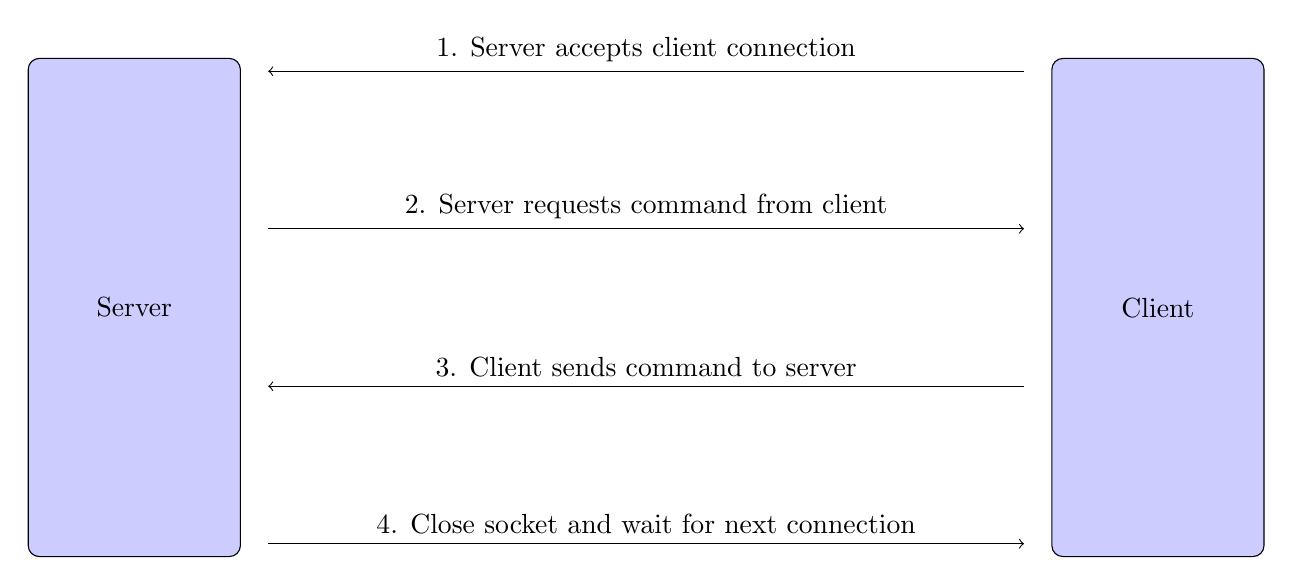
\begin{tikzpicture}[node distance = 2cm, auto]
    % Place nodes
    \node [block] (server){Server};
    \node [block, right of=server] [xshift=11cm] (client) {Client};
    
    %\path [line] (client) [yshift=18cm] -- node [yshift=18cm] {1. Server accepts client connection} (server)
    \coordinate (A) at (1.7,0);
    \coordinate (B) at (11.3,0);
    \draw[<-] ([yshift=3cm] A) -- ([yshift=3cm] B) node [pos=0.5,above] {1. Server accepts client connection};
    \draw[->] ([yshift=1cm] A) -- ([yshift=1cm] B) node [pos=0.5,above] {2. Server requests  command from client};
    \draw[<-] ([yshift=-1cm] A) -- ([yshift=-1cm] B) node [pos=0.5,above] {3. Client sends command to server};
    \draw[->] ([yshift=-3cm] A) -- ([yshift=-3cm] B) node [pos=0.5,above] {4. Close socket and wait for next connection};

\end{tikzpicture}
\newline\newline
The application client was set up so that it only asks the user for a sweet command when the Python server prompts the client for it. The Python server uses an open '0.0.0.0' IP address on the machine running it and then the client uses the specified wireless IP for the server machine. This is inputted into the app on first opening to ensure that the correct IP address is being used for socket connections between the two devices.
\newline\newline
\textbf{User Interface} - The user interface was designed to be simply understood by the user and only require a small amount of setup for the person running the software. The idea of the app is that it would connect to the server on opening, show the main menu and then when Baxter wants a command, the server would send a request to the Java app client, the app would open up the command page, which would prompt the user to record a voice request or enter the sweet numbers they want via touch arrows. The main menu and sweet command page are shown in the images below.
\begin{figure}[H]
    \captionsetup[subfigure]{justification=centering}
    \begin{subfigure}[H]{0.325\textwidth}   
        \centering 
        \includegraphics[width=0.8\textwidth, height=7cm]{ipbootpage.png}
        \caption{Enter IP page.}
        \label{fig:TimeGrasp}
    \end{subfigure}
    \begin{subfigure}[H]{0.325\textwidth}   
        \centering 
        \includegraphics[width=0.8\textwidth, height=7cm]{ipbootpage.png}
        \caption{Main menu page.}
        \label{fig:TimeGrasp}
    \end{subfigure}
    \begin{subfigure}[H]{0.325\textwidth}   
        \centering 
        \includegraphics[width=0.8\textwidth, height=7cm]{sweetchoicepage.png}
        \caption{Choose sweets page.}
        \label{fig:TimeGrasp}
    \end{subfigure}
\end{figure}
When the app is opened, the IP address is entered from the command line printed by the server node. Then the main menu page is viewed until the server wants to receive a customer's command.
\newline\newline
\textbf{Analyse Command} - After the speech has been converted to text using the Google voice recognition API on the device, the text needed to be parsed for a command. The parsing works in a relatively simple way, where it first looks for whether someone has said the words 'blue', 'green' or 'red'. There is also a basic fuzzy search method where it also looks for other words that sound very similar to them. Then after that, the locations of those words are found and then the words before the colours are analysed, to see what number they are. If they are recognised as 'one', 'two', or 'three', then the parser knows how many of each colour the customer wants. This approach works reliably enough and the more people that tested the system, the more changes and extra anomalies were caught in the voice recognition.
\subsubsection{Testing}
\subsection{Customer Recognition}
The next implementation of human interaction was to recognise whether a customer has approached Baxter or not. Then if the customer has approached Baxter for some sweets, Baxter will know and can therefore start the conversation and other aspects of the interaction. The initial idea for the approach was to know when a customer enters and exits the scene, to ideally be further expanded to recognise certain actions, like reach for the sweet bag and exchange money.
\subsubsection{Detect Person}
The first method to detect a person was a very simply devised method, based around background subtraction without any shape recognition on the person whatsoever. Firstly, Baxter would request a ROS node to look for a person. Then Baxter would move his arms out of the way so the head could turn and see a customer enter. The current frame would then be used as the background frame for subtraction. A person would be considered to have entered the scene when a large contour was found entering the scene, seen in \textbf{figure blah}.
\begin{figure}[H]
    \captionsetup[subfigure]{justification=centering}
    \begin{subfigure}[H!]{0.475\textwidth}   
        \centering 
        \includegraphics[width=\textwidth, height=5cm]{convexhulloverlappissues.png}
        \caption{Background person contour.}
        \label{fig:TimeGrasp}
    \end{subfigure}
    \begin{subfigure}[H]{0.475\textwidth}   
        \centering 
        \includegraphics[width=\textwidth, height=5cm]{collisioncorrectdetection.png}
        \caption{Detected contour in image.}
        \label{fig:TimeGrasp}
    \end{subfigure}
\end{figure}
After the person was found, a key part of the recognition would be to make sure the person was in front of Baxter for a set period of time. After the person existed in front of the camera for 40 frames, the node recognised the person as wanting sweets and sent a message back to Baxter to start the interaction. However, if a person did not exist for 40 frames, the program would recognise the contour exiting the scene and therefore carry on waiting for another customer.
\subsubsection{Skeleton Recognition}
Due to time constraints, a working implementation of skeleton recognition could not be implemented by the end of the project. This was partially due to technological issues. To get a skeleton recognition system working, the system would need to implement a second Kinect depth camera. The problem with a second Kinect is that it was difficult to find a place to put the Kinect, due to one Kinect already being on the torso of Baxter looking at the table. This meant that the only place to put a second Kinect was on a tripod away from Baxter, meaning that if Baxter was moved at all on open day, that Kinect would have to be recalibrated each time. The decision to not implement skeleton recognition was then made from a time perspective, as it takes a long time to set up an extra Kinect and calibrate it to work with the system. Due to only having 4 weeks left at the point of discussing this, it was decided it was better to focus on other key features of the project.
\section{System Integration}
\subsection{Node Communication and Custom Service Requests}
\subsection{Control of Vision Processes}
\subsection{Roslaunch Files}
\subsection{System Logic}
%Pages to be referenced for practical applications:
%\newline
%\url{http://docs.opencv.org/3.0-beta/doc/py_tutorials/py_imgproc/py_houghlines/py_houghlines.html#py-hough-lines}
%\url{http://docs.opencv.org/2.4/modules/calib3d/doc/camera_calibration_and_3d_reconstruction.html}
%\url{http://pointclouds.org/documentation/tutorials/region_growing_segmentation.php}
%\newline
%\url{http://pointclouds.org/documentation/tutorials/region_growing_rgb_segmentation.php}
%\newline
%\url{http://wiki.ros.org/tabletop_object_detector}
%\newline
%\url{http://docs.pointclouds.org/trunk/group__sample__consensus.html}
%\newline
%\newline
%\newline
%\newline
~\cite{kinectfusion}
~\cite{objectlabelling}
~\cite{herbrobot}
~\cite{reliablegrasping}